\section{Appendix}
\subsection{How to Store Papers – “Dummy Paper”}\label{app:dummy-paper}
\begin{wrapfigure}{r}{0.5\linewidth}
  \vspace{-1em}
  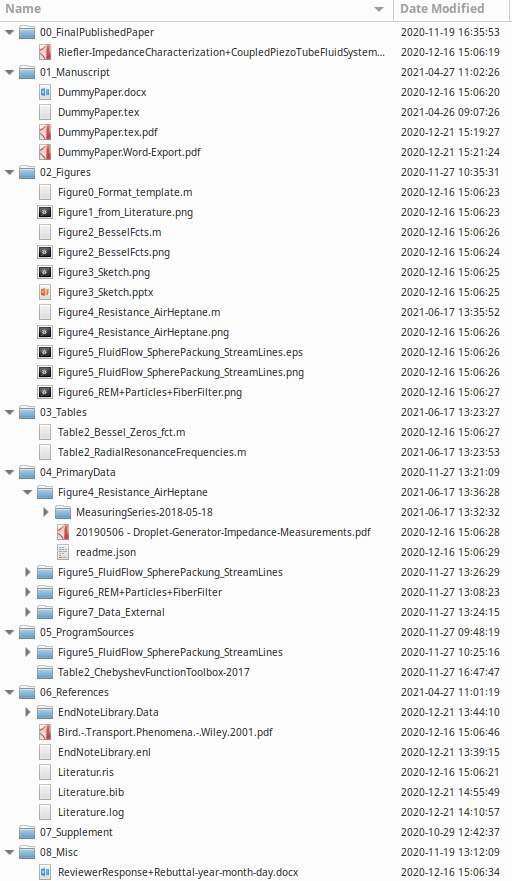
\includegraphics[width=\linewidth]{Figure03_DummyPaperStructureExample4.png}
  \caption{Complete data structure of a dummy paper.}
  \label{fig:dummy-paper}
\end{wrapfigure}
The following screenshot shows a complete data structure of a dummy paper.
You may find this dummy paper on our VT-Server
\href{http://gofile.me/6C5nG/0uMzVrlwb}{here}
(\url{http://gofile.me/6C5nG/0uMzVrlwb}),
together with these guidelines. Basically, the idea is that every data in the
paper, whether it is a figure or a table, can be related to the original source
of the measurement or the simulation. This is realized in the Dummy Paper by
Matlab scripts, but can be done using other means as well (Python, Excel). The
point is: No matter how, but you have to give a relation between the data saved
in the \texttt{‘04\_PrimaryData’} directory and their representation in the
publication. All figures and their generating scripts – here Matlab files – are
given together with the measurement data so that running a Matlab (Octave)
script within that directory generates the according figure. In the end, someone
else can reproduce your results given in your publication. In case of other data
like SEM images for instance, you can refer to them by a PDF generated by the
ELN including a link to the experiment stored there.

The “Dummy Paper” contains a Word and a LaTeX template in
\texttt{‘01\_Manuscript’}. The EndNote or BibTeX literature references are in
\texttt{‘06\_References’}. Both, the EndNote file ‘*.enl’ or the BibTeX file
‘*.bib’, should include links between the references and the freely accessible
PDFs of the papers and books also saved in \texttt{‘06\_References’}.

\subsection{How to Write a DMP}

\subsubsection{Motivation}

A Data Management Plan (DMP) documents the thoughts of an applicant about the
data which will be generated during the applied research project. Research
funders (DFG etc.) expects that publicly promoted projects makes their data
accessible to the public, where a simple publication was sufficient in the past.

There is no unified structure of DMPs due to the vast number of different
research tasks. In the following, the main elements of a DMP from the
TIB Hannover are listed, which can be found also in the recommendation of the
DFG: \\
(\url{https://www.dfg.de/download/pdf/foerderung/grundlagen_dfg_foerderung/forschungsdaten/forschungsdaten_checkliste_de.pdf})

\subsubsection{Elements of a DMP}

\begin{enumerate}[start=0, label=\textbf{\arabic*})]
  \item \textbf{Administrative information}
        \begin{itemize}
          \item Project name
          \item Project participants
          \item Project description
          \item Project ground (doctorate, third party funding, etc.)
          \item Project duration
          \item Version of this DMP
        \end{itemize}
  \item \textbf{Methods and kinds of data gathering}
        \begin{itemize}
          \item Are there primary data generated, or will be secondary data used?
          \item Which data types / formats are generated and processed?
          \item How large are the data?
          \item Which equipment (instruments, hardware, software, etc.)
                will be used?
          \item How are the data organized? (Directory of file oriented
                structure? Version control?)
          \item How is the research process and the data been documented?
          \item Which (technical) standards will be used for
                description/documentation (metadata, classification)?
          \item How are the metadata been generated (e.g. automatically,
                manually, after a guideline, self-defined)?
        \end{itemize}
  \item \textbf{Backup and data safety}
        \begin{itemize}
          \item Where are the data stored?
          \item Which capacity is required?
          \item Interval of data safety?
          \item Are there any protective measures required for sensitive data?
          \item Are there any third party of project partners (e.g. in joint
                projects) who need access to the data?
        \end{itemize}
  \item \textbf{Archiving}
        \begin{itemize}
          \item Which data is archived?
          \item On which data carrier?
          \item Are there any requirements for the operators of the
                infrastructure? E.g. data curation?
          \item Which metadata have to be provided to find the archived data?
          \item Which information is additionally required to understand the
                context of the data?
          \item How long are the data archived?
          \item Are there any legal technicalities for the data archiving?
          \item What are the costs for which service?
        \end{itemize}
  \item \textbf{Data sharing and publication}
        \begin{itemize}
          \item Are there data which must be shared with others?
          \item What are the possible systems for data sharing?
          \item Which metadata and documentation are additionally required for
                third parties to use the data?
          \item Where (data repository, data journal) will the data be
                published, and how (e.g. open access, with embargo time,
                restricted access)?
          \item What are the license condition for the published data?
                (E.g. “CC BY 4.0”)
        \end{itemize}
  \item \textbf{Resources and responsibilities}
        \begin{itemize}
          \item How is the distribution of responsibility governed in this project?
          \item How is responsible for the data management (processes, IT,
                guidelines, formats, monitoring)?
          \item Required personal resources for a successful
                implementation/realization?
          \item What are the costs within the project phase and
                possibly thereafter?
          \item Which infrastructure resources are required, with additionally
                costs?
        \end{itemize}
\end{enumerate}
